%%%%%%%%%%%%%%%%%%%%%%%%%%%%%%%%%%%%%%%%%
% Beamer Presentation
% LaTeX Template
% Version 1.0 (10/11/12)
%
% This template has been downloaded from:
% http://www.LaTeXTemplates.com
%
% License:
% CC BY-NC-SA 3.0 (http://creativecommons.org/licenses/by-nc-sa/3.0/)
%
%%%%%%%%%%%%%%%%%%%%%%%%%%%%%%%%%%%%%%%%%

%----------------------------------------------------------------------------------------
%	PACKAGES AND THEMES
%----------------------------------------------------------------------------------------

\documentclass{beamer}

\mode<presentation> {

% The Beamer class comes with a number of default slide themes
% which change the colors and layouts of slides. Below this is a list
% of all the themes, uncomment each in turn to see what they look like.

%\usetheme{default}
%\usetheme{AnnArbor}
%\usetheme{Antibes}
%\usetheme{Bergen}
%\usetheme{Berkeley}
%\usetheme{Berlin}
%\usetheme{Boadilla}
\usetheme{CambridgeUS}
%\usetheme{Copenhagen}
%\usetheme{Darmstadt}
%\usetheme{Dresden}
%\usetheme{Frankfurt}
%\usetheme{Goettingen}
%\usetheme{Hannover}
%\usetheme{Ilmenau}
%\usetheme{JuanLesPins}
%\usetheme{Luebeck}
%\usetheme{Madrid}
%\usetheme{Malmoe}
%\usetheme{Marburg}
%\usetheme{Montpellier}
%\usetheme{PaloAlto}
%\usetheme{Pittsburgh}
%\usetheme{Rochester}
%\usetheme{Singapore}
%\usetheme{Szeged}
%\usetheme{Warsaw}

% As well as themes, the Beamer class has a number of color themes
% for any slide theme. Uncomment each of these in turn to see how it
% changes the colors of your current slide theme.

%\usecolortheme{albatross}
%\usecolortheme{beaver}
%\usecolortheme{beetle}
%\usecolortheme{crane}
%\usecolortheme{dolphin}
%\usecolortheme{dove}
%\usecolortheme{fly}
%\usecolortheme{lily}
%\usecolortheme{orchid}
%\usecolortheme{rose}
%\usecolortheme{seagull}
%\usecolortheme{seahorse}
%\usecolortheme{whale}
%\usecolortheme{wolverine}

%\setbeamertemplate{footline} % To remove the footer line in all slides uncomment this line
%\setbeamertemplate{footline}[page number] % To replace the footer line in all slides with a simple slide count uncomment this line

%\setbeamertemplate{navigation symbols}{} % To remove the navigation symbols from the bottom of all slides uncomment this line
}

\usepackage{graphicx} % Allows including images
\usepackage{booktabs} % Allows the use of \toprule, \midrule and \bottomrule in tables

%----------------------------------------------------------------------------------------
%	TITLE PAGE
%----------------------------------------------------------------------------------------

\title[Classification of SPD matrices]{Classification of SPD matrices using a Riemannian-based kernel} % The short title appears at the bottom of every slide, the full title is only on the title page

\author{Anna Kuzina} % Your name
\institute[Skoltech] % Your institution as it will appear on the bottom of every slide, may be shorthand to save space
{
Skoltech \\ % Your institution for the title page
\medskip
\textit{anna.kuzina@skoltech.ru} % Your email address
}
\date{\today} % Date, can be changed to a custom date

\begin{document}

\begin{frame}
\titlepage % Print the title page as the first slide
\end{frame}

%\begin{frame}
%\frametitle{Overview} % Table of contents slide, comment this block out to remove it
%\tableofcontents 
%\end{frame}

%----------------------------------------------------------------------------------------
%	PRESENTATION SLIDES
%----------------------------------------------------------------------------------------

%------------------------------------------------
%\section{Notations} % Sections can be created in order to organize your presentation into discrete blocks, all sections and subsections are automatically printed in the table of contents as an overview of the talk
%------------------------------------------------

%\subsection{Subsection Example} % A subsection can be created just before a set of slides with a common theme to further break down your presentation into chunks

\begin{frame}
\frametitle{Motivation}
\begin{itemize}
\item<1-> 	Structural connectome can be seen as symmetric adjacency matrix
\vfill 
\item<2-> Take into account geometry of the data

\end{itemize}

\end{frame}

%------------------------------------------------



\begin{frame}
\frametitle{Basic notations}
\begin{itemize}
	\item $\mathcal{M}(n)$ --- space of $n\times n$ real matrices
	\vfill
	\item $\{S \in \mathcal{M}(n): S^T = S  \}$ --- space of $n\times n$ symmetric matrices
		\vfill
	\item $\{P \in S(n): u^TPu > 0 \; \forall u \in \mathbb{R}^n  \}$ --- space of $n\times n$ SPD matrices
		\vfill
	\item $\exp(S) = C\; \text{diag}(\exp(\lambda_1), \dots, \exp(\lambda_n) ) \; C^T  \in P(n)$
		\vfill
	\item $\log(P) = C\; \text{diag}(\log(\lambda_1), \dots, \log(\lambda_n) ) \; C^T \in S(n)$
		\vfill
	\item $P^{\frac12}$ --- symmetric matrix $A$, s.t. $AA = P$
\end{itemize}

\end{frame}

%------------------------------------------------

\begin{frame}
\frametitle{Riemannian manifold}
\begin{itemize}
\item Smooth manifold
\item Tangent finite-dimensional Euclidean space at every point with inner product $g_P$
\item $g_P$, Riemannian metric, varies smoothly from point to point

\end{itemize}
 \hfill 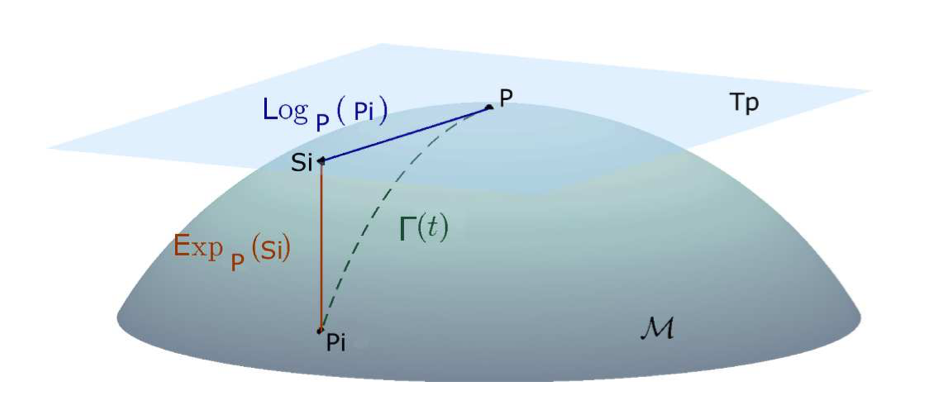
\includegraphics[scale=0.5]{manifold.png}
\end{frame}

%------------------------------------------------


\begin{frame}
\frametitle{Exponential map}
\begin{block}{Exponential mapping}
	\begin{equation*}
	 \exp_P(S_i)  = P_i = P^{\frac12} \exp(P^{-\frac12}S_iP^{-\frac12})P^{\frac12}
	\end{equation*}
\end{block}

\begin{block}{Logarithmic mapping}
	\begin{equation*}
	\log_P(P_i)  = S_i = P^{\frac12} \log(P^{-\frac12}P_iP^{-\frac12})P^{\frac12}
	\end{equation*}
\end{block}
\end{frame}

%------------------------------------------------

\begin{frame}
\frametitle{Riemannian metrics}

\begin{block}{Inner product}
	\begin{equation*}
	\langle S_1, S_2 \rangle_P = \text{Tr}(S_1 P^{-1}S_2 P^{-1})
	\end{equation*}
\end{block}

\begin{block}{Norm}
	\begin{equation*}
	\|S \|_P^2 = \text{Tr}(S P^{-1}SP^{-1})
	\end{equation*}
\end{block}

$P = I:$
	\begin{equation*}
 \|S\|_I^2 = \text{Tr}(S^2) =  \text{Tr}(S^TS) = \|S\|_F^2 = \|\text{vect}(S)\|_2^2
 \end{equation*}
 \begin{equation*}
 \text{vect}(S) = \left[ S_{1,1}, \sqrt{2}S_{1,2}, S_{2,2}, \sqrt{2}S_{1,3} ,  \sqrt{2}S_{2,3}, S_{3,3}, \dots, S_{n,n}  \right]^T
 \end{equation*}
 
\end{frame}
%------------------------------------------------
\begin{frame}
\frametitle{Riemannian Geodesic distance}

\begin{block}{}
	The geodesic --- shortest path between two points\\
	Riemannian distance --- length of the geodesic
\end{block}
	\uncover<2->{
\begin{block}{}
		\begin{equation*}
	\Gamma(t): [0,1] \rightarrow P(n)
	\end{equation*}
	\begin{equation*}
	L(\Gamma(t)) = \int_{0}^{1} \|\dot{\Gamma(t)}\|_{\Gamma(t)}dt
	\end{equation*}
\end{block}}
\begin{columns}[c] 
	\uncover<2->{
\column{.45\textwidth} % Left column and width
 $S_i$ can be seen as derivative of the geodesic between $P$ and $P_i$ at point $t=1$}
\column{.5\textwidth} % Right column and width
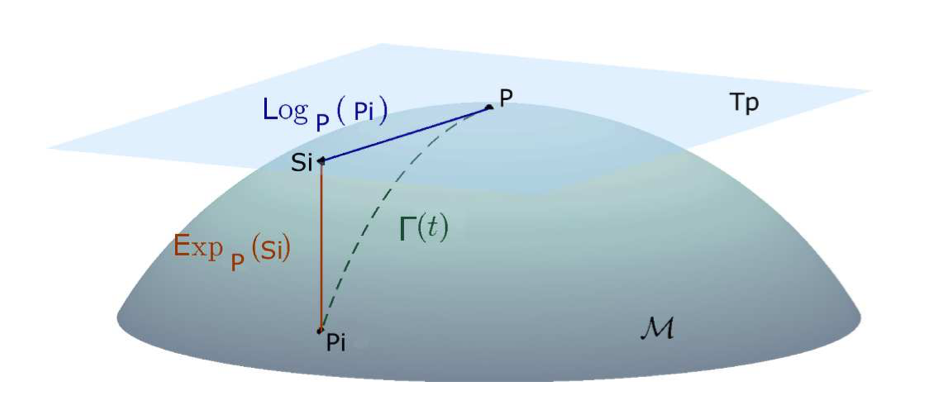
\includegraphics[scale=0.45]{manifold.png}
\end{columns}

\end{frame}


%------------------------------------------------

\begin{frame}
\frametitle{Riemannian distance}
\begin{block}{}
\begin{equation*}
	\sigma_R (P_1, P_2) = \|\log(P_1^{-1}P_2)\|_F = \left( \sum \log^2\lambda_i \right)^{\frac12}
\end{equation*}
\end{block}
\end{frame}

%------------------------------------------------

\begin{frame}
\frametitle{ Classification in the Riemannian manifold}
\begin{itemize}
	\item Minimum distance to Riemanian Mean
\begin{block}{Geometric mean}
	\begin{equation*}
	P^* = \arg\min_P \sum_{i=1}^{m}\sigma^2_R(P, P_i)
	\end{equation*}
\end{block}
\vfill
\item kNN with Riemannian distances
\end{itemize}

\end{frame}

%------------------------------------------------



\begin{frame}
\frametitle{Kernel Approach}

\begin{block}{Mapping function}
	\begin{equation*}
		\phi (P_i) = \log_{P^*}(P_i)
	\end{equation*}
\end{block}
\begin{block}{Riemannian base kernel}
	\begin{equation*}
 k_R(P_i,P_j) = \langle 	\phi (P_i), 	\phi (P_j)\rangle_{P^*} = \text{Tr}( \log_{P^*}(P_i)P^{*-1} \log_{P^*}(P_j)P^{*-1}) = 
	\end{equation*}
	\begin{equation*}
 =	\text{Tr}( \log (P^{*-\frac12}P_i P^{*-\frac12}) \log (P^{*-\frac12}P_j P^{*-\frac12})) =	\text{Tr}(\tilde{P_i}\tilde{P_j}) = 
	\end{equation*}
	\begin{equation*}
	= \langle \tilde{P_i},\tilde{P_j} \rangle_F =  \text{vect}(\tilde{P_i})^T  \text{vect}(\tilde{P_j}) =  \langle  \text{vect}(\tilde{P_i}), \text{vect}(\tilde{P_j}) \rangle_2
	\end{equation*}
\end{block}

\end{frame}

%------------------------------------------------


\begin{frame}
\frametitle{Reference point}
	\begin{equation*}
k_R(P_i,P_j) = \text{Tr}( \log (P^{*-\frac12}P_i P^{*-\frac12}) \log (P^{*-\frac12}P_j P^{*-\frac12})) =	\text{Tr}(\tilde{P_i}\tilde{P_j})
\end{equation*}
\uncover<2->{
\begin{block}{log-Euclidean kernel}
	$$
	P^* = I
	$$
\begin{equation*}
  k_{LE}(P_i,P_j)  = \text{Tr}(\log(P_i)\log(P_j))
\end{equation*}
\end{block}}
\uncover<3->{
\begin{block}{Geometric mean}
\begin{equation*}
	P^* = \arg\min_P \sum_{i=1}^{m}\sigma^2_R(P, P_i)
\end{equation*}	
\end{block}}

\end{frame}

%------------------------------------------------


\begin{frame}
\frametitle{From SI to SPD}
\begin{enumerate}
\item Laplacian of the SI adjacency matrix  --- SPSD matrix
\begin{equation*}
L_S = D_S - S
\end{equation*}
\vfill
\uncover<2->{
\item Add regularization
\begin{equation*}
	P  = L_{S} + \lambda I, \; \lambda > 0
\end{equation*}}
\end{enumerate}

\end{frame}

%------------------------------------------------


\begin{frame}
\frametitle{References}
\footnotesize{
\begin{thebibliography}{99} % Beamer does not support BibTeX so references must be inserted manually as below
\bibitem[Smith, 2012]{p1} M. Moakher (2005)
\newblock Symmetric Positive-Definite Matrices: From Geometry to Applications and Visualization
	
\bibitem[Smith, 2012]{p1} A. Barachant et al. (2010)
\newblock Riemannian Geometry Applied to BCI Classification

\bibitem[Smith, 2012]{p2} A. Barachant et al.(2012)
\newblock Multiclass Brain-Computer Interface Classification by Riemannian Geometry

\bibitem[Smith, 2012]{p3} A. Barachant et al. (2012)
\newblock Classification of covariance matrices using a Riemannian-based kernel for BCI applications

\bibitem[qq]{p4}  A. Pimkin, M. Belyaev et al. (2017)
\newblock Classification of brain network structures using analysis of symmetric semidefinite matrices

\end{thebibliography}
}
\end{frame}

%------------------------------------------------

\begin{frame}
\Huge{\centerline{The End}}
\end{frame}

%----------------------------------------------------------------------------------------

\end{document} 